% !TEX program = pdflatex
%%%%%%%%%%%%%%%%%%%%%%%%%%%%%%%%%%%%%%%%%
% Structured General Purpose Assignment
% LaTeX Template
%
% This template has been downloaded from:
% http://www.latextemplates.com
%
% Original author:
% Ted Pavlic (http://www.tedpavlic.com)
%
% Note:
% The \lipsum[#] commands throughout this template generate dummy text
% to fill the template out. These commands should all be removed when
% writing assignment content.
%
%%%%%%%%%%%%%%%%%%%%%%%%%%%%%%%%%%%%%%%%%

%----------------------------------------------------------------------------------------
%	PACKAGES AND OTHER DOCUMENT CONFIGURATIONS
%----------------------------------------------------------------------------------------

\documentclass{article}

\usepackage{fancyhdr} % Required for custom headers
\usepackage{lastpage} % Required to determine the last page for the footer
\usepackage{extramarks} % Required for headers and footers
\usepackage{graphicx} % Required to insert images
\usepackage{subcaption}
\usepackage{lipsum} % Used for inserting dummy 'Lorem ipsum' text into the template

\usepackage[utf8]{inputenc}
\usepackage[ngerman,english]{babel}
\usepackage[T1]{fontenc}
\usepackage{breakurl}
\usepackage[hyphens]{url}
\usepackage{color}
\usepackage{float}
\usepackage[hidelinks]{hyperref}
\usepackage{tabularx}
\usepackage{enumitem}
\usepackage{color, colortbl}
\usepackage[super]{nth}
\usepackage{wrapfig}
\usepackage{amsmath}
\usepackage{amssymb}
\usepackage{booktabs}
\usepackage{titlesec}

\usepackage[
	backend=biber,
	style=numeric-comp,
	natbib=true,
	url=false,
	doi=false,
	eprint=false,
	sorting=none,
	isbn=false]
	{biblatex}

\titleformat{\paragraph}
{\normalfont\normalsize\bfseries}{\theparagraph}{1em}{}
\titlespacing*{\paragraph}
{0pt}{3.25ex plus 1ex minus .2ex}{1.5ex plus .2ex}

\bibliography{references}

\addto\captionsenglish{%
  \renewcommand{\contentsname}%
    {Table of Contents}%
}

% Margins
\topmargin=-0.45in
\evensidemargin=0in
\oddsidemargin=0in
\textwidth=6.5in
\textheight=9.0in
\headsep=0.25in

\linespread{1.1} % Line spacing
% Set up the header and footer
\pagestyle{fancy}
\lhead{} % Top left header
\chead{} % Top center header
\rhead{\firstxmark} % Top right header
\lfoot{\lastxmark} % Bottom left footer
\cfoot{} % Bottom center footer
\rfoot{Page\ \thepage\ of~\pageref{LastPage}} % Bottom right footer
\renewcommand\headrulewidth{0.4pt} % Size of the header rule
\renewcommand\footrulewidth{0.4pt} % Size of the footer rule

\setlength\parindent{0pt} % Removes all indentation from paragraphs

\begin{document}
\setcounter{tocdepth}{2} % No subsubsections


%----------------------------------------------------------------------------------------
% TITLE PAGE
%----------------------------------------------------------------------------------------
\pagenumbering{gobble}
% \maketitle
\begin{titlepage}
  \centering
\includegraphics[width=5cm]{figures/tumlogo}

  \vspace{2.5cm}
  \Huge{Network Security} \\
  \vspace{0.1in}\huge{Summary}\\

  \Large
  \vspace{1.5cm}
  \begin{tabularx}{9cm}{r l}
    Author: & Thomas Pettinger\\
  \end{tabularx}

  \vfill
  \textbf{2017--03--02} \\
  \vspace{0.3in}\normalsize{Network Security}\\
  \vspace{0.03in}\normalsize{\textsc{Technische Universität München}}\\
  \vspace{1cm}

\end{titlepage}
%----------------------------------------------------------------------------------------


\newpage
\thispagestyle{empty}
\tableofcontents

\newpage
\pagenumbering{arabic}

%!TEX root = ../report.tex

\section{Introduction}

\subsection{Attacks and Attack Detection}
Attacks can have different impacts on the target.
Disruptive attacks try to fully deny the service (DoS) of the victim whereas degrading ones only occupy parts of the resources.
A DoS attack can also executed distributed, a so called DDoS.
Attackers might also try to gain confidential data or control the target system.
Port scans can be used to gain information about the network topology, operating systems and applications or application versions.\\

To be able to tell if a system is under attack, different measures can be taken at different points in the system.\\
Host intrusion detection systems (HIDS) are located on the host system.
This enables easy detection using information available on the potential victim system but it has to be present on every system (expensive deployment) and the attack actually reaches the victim and is not detected in advance.
Network intrusion detection systems (NIDS) lay on the network layer which enables the detection of attacks before they reach the host.\\
One of the detection methods available is knowledge-based detection.
Known signatures of attacks are compared to the actual traffic and if the patterns match an alarm is raised.
This only detects known attacks though.
To improve this shortcoming, anomaly detection in traffic, protocol or applciaiton behavior can be used.
Anomalies can be detected with different metrics in mind.
A very simple one might be the number of request, but this does not take legitimate change in traffic into account.
A better approach is using cumulative sums which are low if the average is small or whenever only small amounts of values are large but grows if the amount of large values grows in a certain point in time.
The disadvantage of anomaly detection though is that oftentimes the rate of false-positives is high.\\
Detecting attacks is not easy and network monitory often comes at a cost.
It is important though especially in large systems when the attack surface grows.
The challenge is to find a good compromise between security and performance.

\subsection{Attacker Model and Locations}
We generally assume the attacker to be (in) the network.
They can perform any active or passive attack but cannot break cryptographic primitives.
Active attacks are attacks where some influence is measurable e.g.\ a delay, modifications or replays whereas a passive attack simply stands for eavesdropping messages.
This model is called the Dolev-Yao attacker model.\\

Attackers can be located on different parts of the network and depending on this location different attacks are possible.
If the attacker is close to you they are able to perform active attacks like message modifications on you.
This can be circumvented by communicating over a secure tunnel though.
If the attacker is close to your servers, timing attacks are possible where attackers can measure how long certain operations take to break into the system.
The last possibility is that the attacker is somewhere in the Internet.
Since the end user has no control over how packets are routed, attackers can modify the path they take for example.

\subsection{Security Goals}
\begin{description}
  \item[Data Integrity] No improper or unauthorized change of data
  \item[Confidentiality] Concealment of information
  \item[Availability] Services should be available and function correctly
  \item[Authenticity] Entity is who she claims to be
  \item[Accountability] Identify the entity responsible for any communication event
  \item[Controlled Access] Only authorized entities can access certain services or information
\end{description}

\subsection{Threads}
We define a thread in a communication as any possible event or sequence of actions that might lead to a violation of one or more security goals.
The actual realization of a thread is then called attack.\\

Different threads are possible:
\begin{itemize}[noitemsep, topsep=0pt]
  \item \textbf{Masquerade}: An entity claims to be another entity (also called ``impersonation'')
  \item \textbf{Eavesdropping}: An entity reads information it is not intended to read
  \item \textbf{Loss or Modification of (transmitted) Information}: Data is being altered or destroyed
  \item \textbf{Denial of Communication Acts (Repudiation)}: An entity falsely denies its participation in a communication act
  \item \textbf{Forgery of Information}: An entity creates new information in the name of another entity
  \item \textbf{Sabotage/Denial of Service}: Any action that aims to reduce the availability and / or correct functioning of services or systems
  \item \textbf{Authorization Violation:}: An entity uses a service or resources it is not intended to use
\end{itemize}

\newpage

%!TEX root = ../report.tex

\section{Language-theoretic Security}
Communication protocols define the procedure and the format of exchanged messages.
If two communication partners speak the same protocol it is not necessarily given that they have the same understanding though.
Different problems may arise which result in some guidelines to avoid them:

\begin{description}
  \item[Full input recognition] Programmers usually assume well formed input where in reality the input is controlled by the attacker.
    For this reason every input should be checked if it fulfills the expectations of valid inputs.
  \item[Only Type 2 or 3 of Chomsky Hierarchy grammars for inputs]
    Do not define turing-complete protocols because recognition of the input and testing the equivalence of implementations is undecidable.
    \begin{figure}[h]
      \centering
      \begin{tabular}{l l l}
        Grammar & Language & Recognized by\\
        \midrule
        Type 3 & Regular & Finite state automaton\\
        Type 2 & Context-free & Pushdown automaton\\
        Type 1 & Context-sensitive & Some weird stuff\\
        Type 0 & recursively enumerable & Turing machine\\
      \end{tabular}
      \caption{Chomsky Hierarchy of Languages}
    \end{figure}
  \item[Reduce computing power] Reduce the computing power exposed to the outside.
    Computing power that is not there can not be exploited.
    This also includes defining protocols only in type 2 or 3 languages since parsing types 0 and 1 requires large or potentially unlimited amounts of computing.
  \item[Same interpretation of messages] All participants of a communication should interpret messages the same way.
    For this parsers have to be equivalent which is only decidable for type 2 and 3.
\end{description}


\newpage

%!TEX root = ../report.tex

\section{Firewalls and Security Policies}
We define a system as secure if, started in an allowed state, always stays in states that are allowed.

\subsection{The three Security Components}
\begin{itemize}
  \item \textbf{Requirements} define security goals
  \item \textbf{Policy} are rules to implement the requirements
  \item \textbf{Mechanisms} enforce the policy
\end{itemize}

\subsection{Network Firewalls}
Firewalls provide \textbf{controlled access} at the network level to resources.
They are usually deployed where a protected subnet is connected to a less trusted network like the internet (c.f.\ Figure~\ref{fig:firewall_placement}).
From the firewall's point of view, there are incoming and outgoing packages on all interfaces.
These can be filtered using two different strategies.\\
\textbf{Whitelisting}, which is considered as the best practice, has the default behavior of denying all packets and allowing only explicitly permitted ones whereas \textbf{blacklisting} allows everything except blocked packets.


\begin{figure}[h]
  \centering
  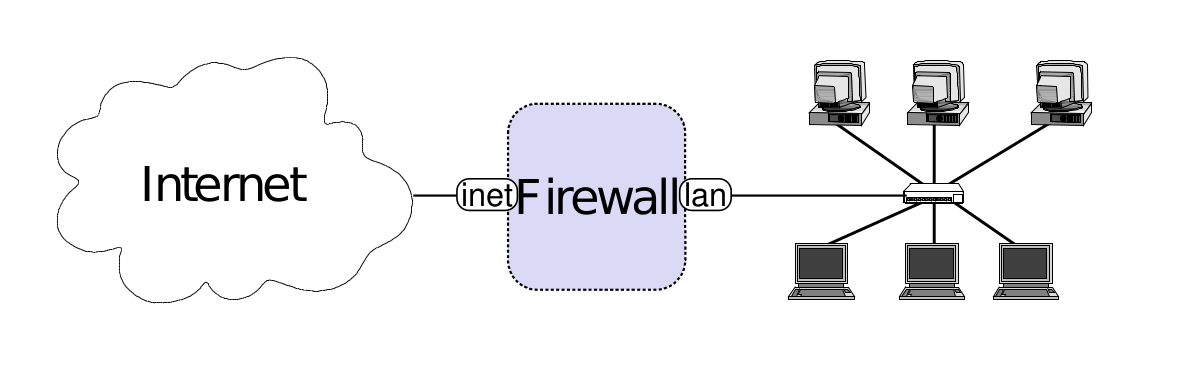
\includegraphics[width=.8\textwidth]{figures/firewall_placement.png}
  \caption{Firewall Placement}\label{fig:firewall_placement}
\end{figure}

\subsubsection*{Configuring Firewalls}
Firewalls are configured with rulesets which are traversed sequentially until a matching one is found.
Those rules are composed of a matching condition and an action.
Possible actions are for example accept, drop, reject or log.
The matching conditions are a bit more complex.
They include the incoming interface, several layer 2 to 4 packet fields (srcMAC, dstMAC, srcIP, dstIP, prot, srcPort, dstPort, flags,\dots), states (in case of stateful matching) and other relevant conditions.

\subsubsection*{Stateful Firewalls}
Stateful Firewalls keep states of connections with the help of IP-5-Tuples (srcIP, dstIP, protocol, srcPort, dstPort).
A new state is generated when a packet with a new tuple arrives which transitions from NEW to ESTABLISHED state.
It is usually advisable to put more frequently used rules to the top of the firewall, i.e.\ matching established connections (new connections are rarer) and to check that ports are above the well defined port range ($\geq 1024$).
Figure~\ref{fig:stateful_firewall} shows an example of a stateful firewall configuration.
\begin{figure}[h]
  \centering
  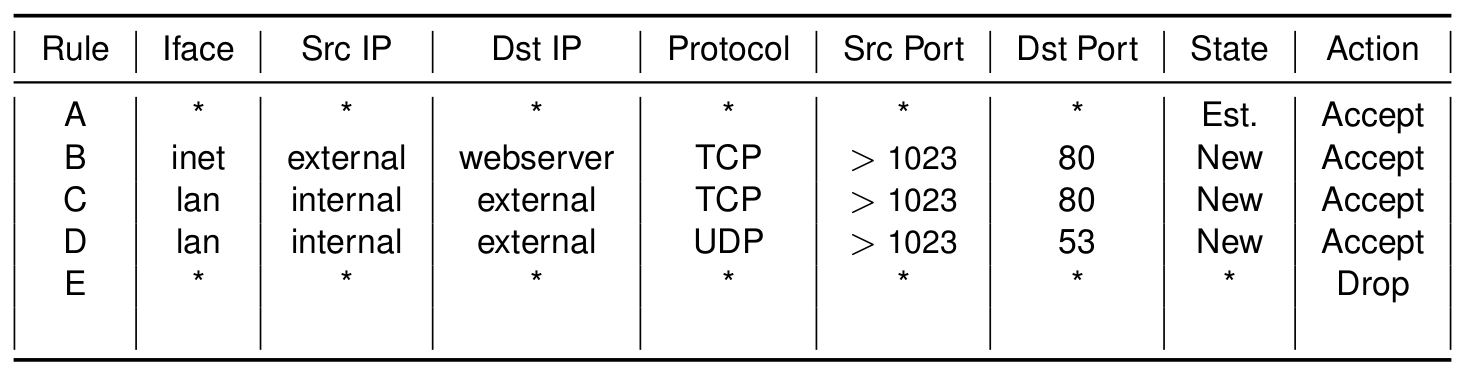
\includegraphics[width=.8\textwidth]{figures/stateful_firewall.png}
  \caption{Stateful Firewall Configuration}\label{fig:stateful_firewall}
\end{figure}

\subsubsection*{Stateless Firewalls}
Stateless firewalls do not generate states for incoming connections but only operate on single packets since keeping states is expensive and needs fast memory.
For this reason lookup times are in $\mathcal{O}(\#rules)$ which, for large $\#rules$ is slower than stateful filtering ($\mathcal{O}(1)$).
For small $\#rules$ stateless filtering is faster though due to the lack of memory writes.
It is also more complex to configure which makes the approach more error prone.
An example for a stateless ruleset is shown in Figure~\ref{fig:stateless_firewall}.
\begin{figure}[h]
  \centering
  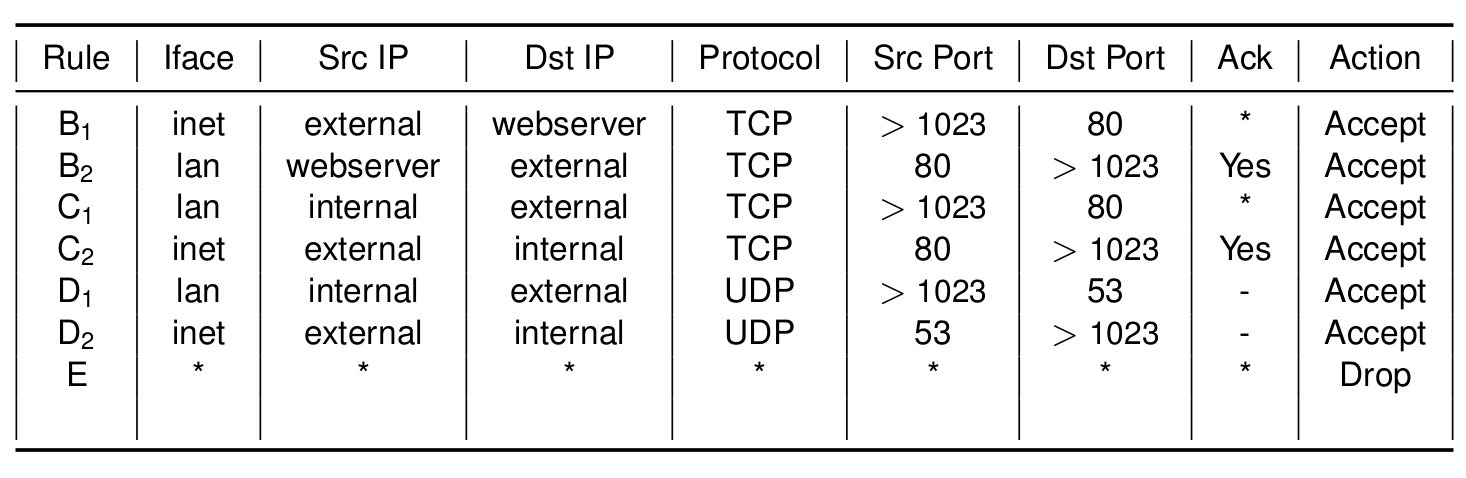
\includegraphics[width=.8\textwidth]{figures/stateless_firewall.png}
  \caption{Stateless Firewall Configuration}\label{fig:stateless_firewall}
\end{figure}

Stateless firewalls usually look at the ACK flag of TCP connection to determine approximately if connections are new or established.
When a SYN/ACK packet is sent as first packet of a connection, the firewall will pass it but the host will drop it if implement properly.

\subsubsection*{Spoofing Protection}
Spoofing is the forgery of IP addresses by filling the source IP field with another IP than one's own.
Spoofing protection then allows only IP addresses that belong to you on outgoing connections.
For incoming traffic this is more difficult since we can not determine where the packet actually came from so we are only able to block our and special purpose IPs.

\subsubsection*{Common Errors}
\begin{itemize}[noitemsep, topsep=0pt]
  \item How is your firewall management interface reachable?
  \item What is allowed over the Internet?
  \item IPv4 and IPv6?
  \item Outbound rule ANY? (c.f.\ spoofing)
  \item Policy’s vs. Firewalls understanding of Inbound and Outbound?
  \item Shadowing: unreachable firewall rules
\end{itemize}

\subsubsection*{What Firewalls cannot do}
\begin{itemize}[noitemsep, topsep=0pt]
  \item can’t protect against malicious insiders
  \item can’t protect against connections that don’t go through it
  \item can’t protect against completely new threats
  \item can’t fully protect against viruses
  \item does not perform cryptographic operations, e.g.\ message authentication
  \item can’t set itself up correctly
\end{itemize}

\subsubsection*{Bastion Hosts}
A bastion host is a host that is more exposed to the hosts of an external network than the other hosts of the network it protects.
When configuring, one should keep in mind that it might get compromised so do things like disabling SSH password login, do not allow it to sniff internal traffic or disable user accounts.

\subsubsection*{Firewall Architectures}
\begin{description}
  \item[Simple Packet Filter Architecture] Packet filtering is done through a filtering router or firewall with two interfaces.
    \begin{figure}[H]
      \centering
      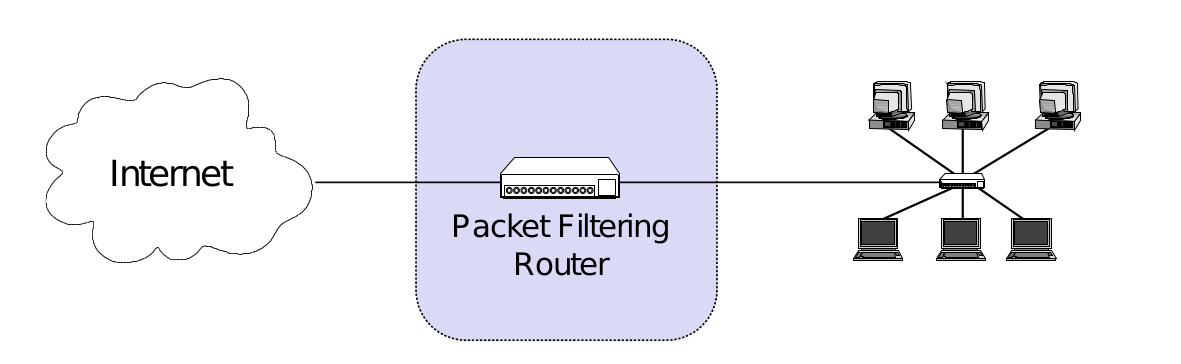
\includegraphics[width=.8\textwidth]{figures/firewall_simple_packet_filter_architecture.png}
    \end{figure}
  \item[Dual-Homed Host Architecture] The bastion host is part of two networks and is firewall and application proxy.
    Disadvantage: bastion host is bottleneck
    \begin{figure}[H]
      \centering
    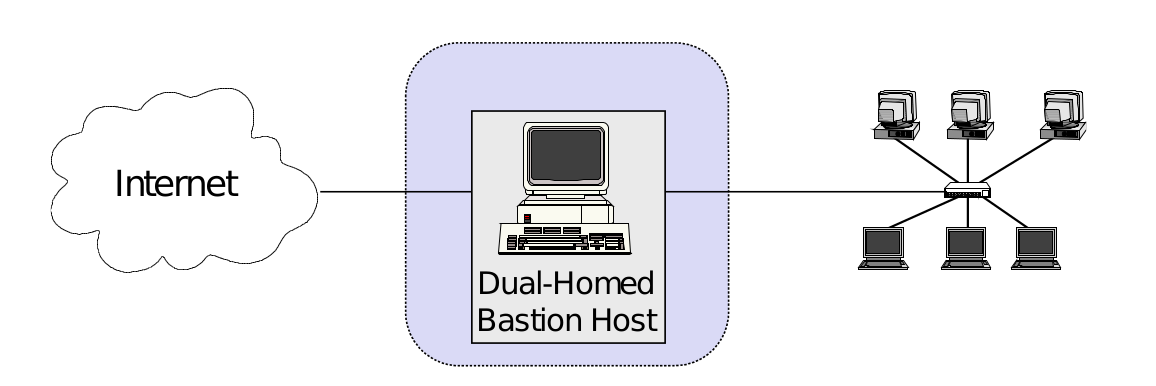
\includegraphics[width=.8\textwidth]{figures/firewall_dual-homed_host_architecture}
    \end{figure}
  \item[Screened Host Architecture] The bastion host is proxy, located in the internal network and thus protected by the firewall.
    \begin{figure}[H]
      \centering
      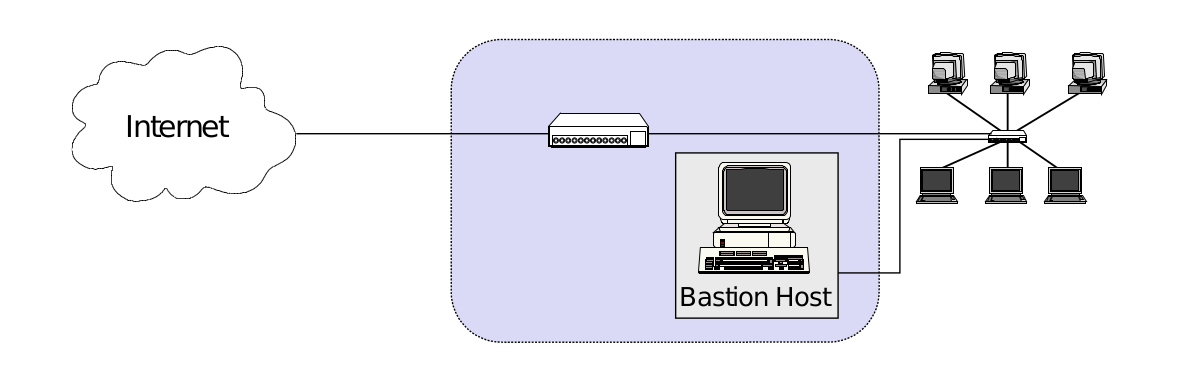
\includegraphics[width=.8\textwidth]{figures/firewall_screening_host_architecture.png}
    \end{figure}
  \item[Screened Subnet Architecture - DMZ] A demilitarized zone (DMZ) is configured hosting the bastion host (proxy) and publicly accessible servers.
    The second packet filter is an additional protection measurement in case the DMZ gets compromised.
    \begin{figure}[H]
      \centering
      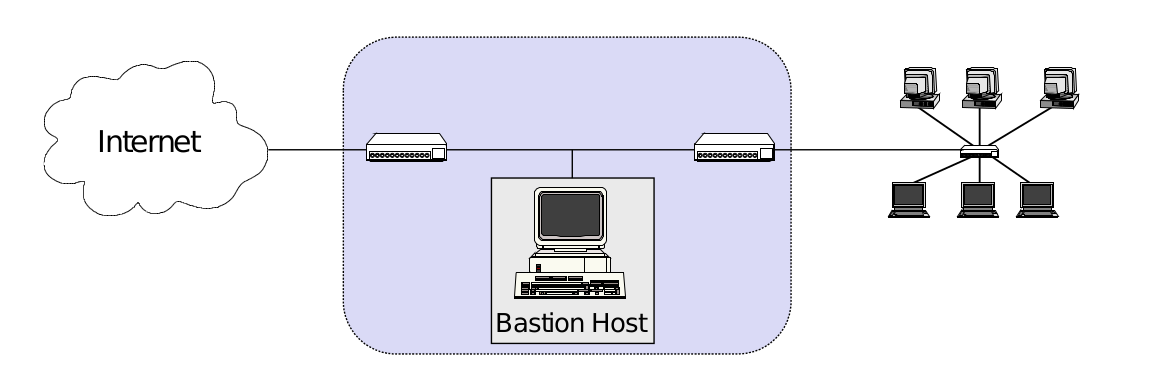
\includegraphics[width=.8\textwidth]{figures/firewall_screened_subnet_architecture.png}
    \end{figure}
\end{description}

\newpage

%!TEX root = ../report.tex

\section{TCP SYN Cookies}

\subsection{TCP SYN Flood Attack}
During an TCP SYN Flood Attack an attacker sends large amounts of packets with spoofed source addresses to the victim.
This fills up their connection table with half open connections (sequence numbers) which results in legitimate users not being able to establish new TCP connections.
A solution for this are TCP SYN cookies.

\subsection{TCP SYN Cookies}
TCP SYN Cookies are particularly chosen initial sequence numbers $\alpha = h(S_{SYN},K)$ where $K$ is a secret key, $S_{SYN}$ the source address of the SYN packet and $h$ a cryptographic hash function.
On arrival of the ACK message, Bob calculates $\alpha$ again and checks if the ACK number is correct ($\alpha + 1$).
This process is shown in Figure~\ref{fig:tcp_syn_cookies}.
\begin{figure}[h]
  \centering
  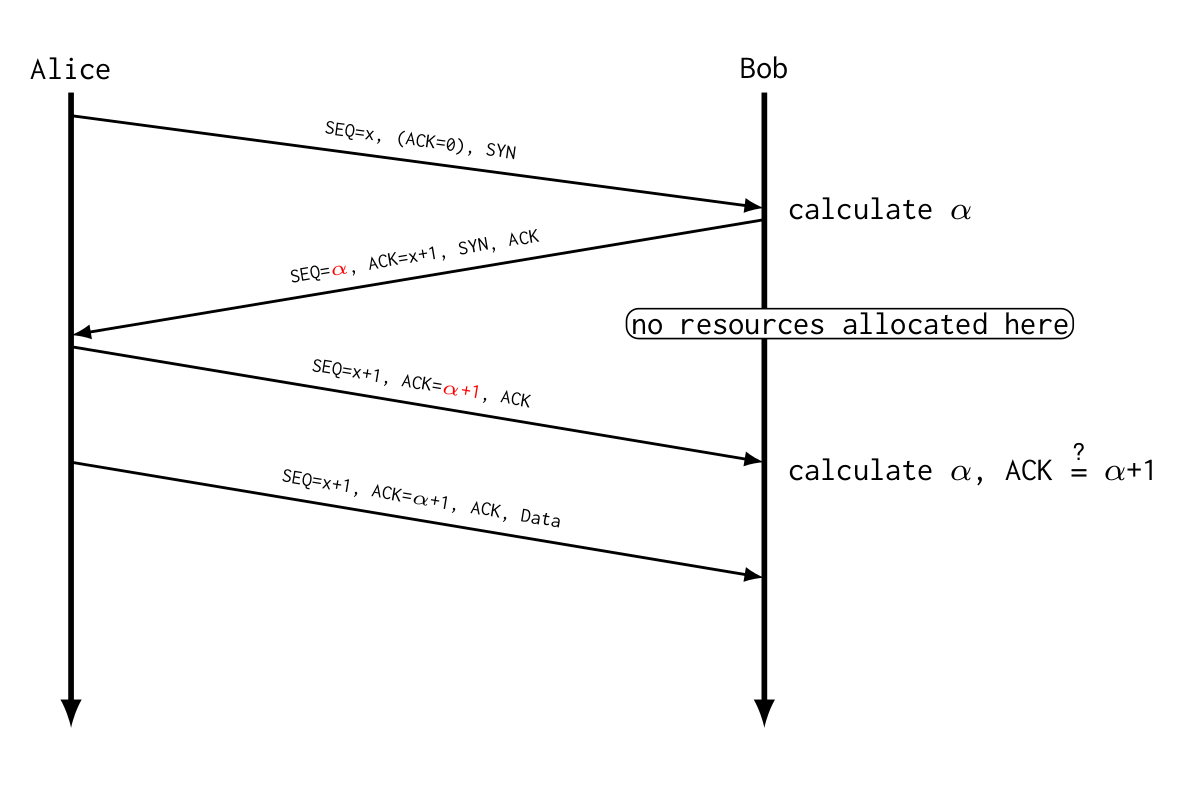
\includegraphics[width=.6\textwidth]{figures/tcp_syn_cookies.png}
  \caption{TCP SYN Cookies}\label{fig:tcp_syn_cookies}
\end{figure}

\begin{minipage}[t]{0.49\textwidth}
  \textbf{Pros}
  \begin{itemize}[topsep=0pt,noitemsep]
    \item No resource allocation after SYN packets
    \item Client does not have to be aware of the server using SYN cookies
    \item No changes in the TCP protocol necessary
  \end{itemize}
\end{minipage}
\begin{minipage}[t]{0.49\textwidth}
  \textbf{Cons}
  \begin{itemize}[topsep=0pt, noitemsep]
    \item Calculating $\alpha$ may be CPU consuming (Linux implementation: CPU local with high cashing efficiency)
    \item TCP options (like large windows size) cannot be negotiated (Linux implementation: window size hacked into cookie, SYN cookies only enabled if a threshold of connections is exceeded)
    \item Efficient implementations might be vulnerable to cryptoanalysis (Linux implementation: SHA used, counter updated every minute)
  \end{itemize}
\end{minipage}
\vspace{20pt}


\newpage

%!TEX root = ../report.tex

\section{Cryptography}
Cryptography is the field of science which is concerned with secure communication.
It provides cryptographic schemes to achieve confidentiality (ciphers) and authenticity (message authentication codes).

\subsection{Security of Cryptographic Schemes}
A secure scheme is defined as a scheme, for which it is impossible for a probabilistic polynomial adversary to break it with at most negligible probability.
Negligibility is defined as $f(n) < \frac{1}{p(n)}$ for a polynomial p and sufficiently large n, e.g.\ $f(n) = \frac{1}{2^n}$.

Kerckhoff's principle states that the cipher method must not be required to be secret, and it must be able to fall into the hands of the enemy without inconvenience.
Thus only the key needs to be secret.\\

It is advisable to use only standardized schemes from libraries and to RTFM (read the fucking manual) because implementing own schemes has a lot of pitfalls and is more often or almost always done wrong.
One also has to keep in mind, that encryption alone does not imply that the system is secure, often integrity and authenticity are more important than confidentiality.
And also do not forget key management.

\subsubsection*{Security of Ciphers}
We define a cipher as secure if it is impossible for attackers to recover they key, the entire or even any character of the plaintext from the ciphertext.
This is the case if the ciphertext is indistinguishable from a random string with uniform distribution of the character probabilities.

\subsection{Hash Functions}
Hash functions are functions which take inputs of arbitrary and transform them to a fixed length output.
Cryptographic hash functions must also have the following properties:
\begin{itemize}
  \item \textbf{Pre-image resistance}: It is infeasible to find an $x'$ s.t.\ $H(x') = H(x)$ for given $H(x)$ and randomly chosen $x$.
  \item \textbf{Second pre-image resistance}: It is infeasible to find an $x' \neq x$ s.t.\ $H(x') = H(x)$ for a given $x$.
  \item \textbf{Collision resistance}: It is infeasible to find $x' \neq x$ s.t.\ $H(x) = H(x')$.
\end{itemize}
This implies that the that cryptographic hash functions have to be one-way functions.
These are functions where it is computationally infeasible to calculate the inverse function.\\

Cryptographic has functions can be used for authentication, pseudo-random number generation ($b_0 = seed$ and $b_i+1 = H(b_i|seed)$) or encryption (e.g.\ in OFB).
An example is SHA-3.

\subsection{Randomness}
We define randomness as unpredictability or entropy.
A measure for entropy is the Shannon information entropy calculation
\begin{equation*}
  H(X) = - \sum_x P(X = x)ln_2(P(X=x))
\end{equation*}
where X is a random variable outputting a sequence of $n$ bits.
This entropy and thus randomness is maximized ($H(X) = n$) if bits are uniformly distributed.\\

Randomness is an important part of cryptography, e.g.\ for generating keys.
In computing, there is no true randomness though since computers are deterministic.
For this reason, cryptographically secure pseudo random number generators (CSPRNG) are used which are deterministic algorithms that take truly random, binary input sequences (seed) and output a random-looking sequence of numbers.
These unpredictable inputs might either be values resulting from physical phenomena (time between emission of particles, thermal noise of semiconductor, \dots) or from software (elapsed time between keystrokes, packet interarrival times, \dots).


\subsection{Symmetric Cryptography}
In symmetric encryption two communication partners Alice and Bob share a secret key that is used for encryption and decryption or message authentication.

We use the following terminology:
\begin{itemize}[noitemsep, topsep=0pt]
  \item $\leftarrow$ non-deterministic assignment
  \item $:=$ deterministic assignment
  \item Key $k \leftarrow Gen(1^n)$
  \item Plaintext $m = Dec_k(c)$
  \item Ciphertext $c = Enc_k(m)$
  \item $Dec_k(Enc_k(m)) = m$
\end{itemize}

\subsubsection{One-Time-Pad (OTP): A Perfect Cypher}
For the OTP a perfectly random bitstream $opt$ with the length of the message to encode is needed.
Then the encryption operation is defined as $Enc_{otp}(m) = m \oplus otp$ and the decryption operation as $Dec_{otp}(c) = c \oplus otp$
For the OTP to be perfectly secure, the key must only be used once which is impractical in the real world where we usually want $length(k) \ll length(m)$ and thus reusable keys.

\subsubsection{Attacking Symmetric Ciphers}
The goals of attacks on ciphers is to learn something about $m$ given a $c$.
Getting any information about $k$ from an attack is also considered a successful one.\\

To analyze the security, cryptography uses attack games where $\mathcal{C}$ is the challenger and $\mathcal{A}$ the adversary.

Possible attack scenarios are listed in the following, of which some are explained more precisely below:
\begin{itemize}[noitemsep, topsep=0pt]
  \item Ciphertext-only-attack: attacker knows $c$
  \item Known-plaintext-attack: For a fixed $k$, the attacker got a pair $(m, c)$ and tries to learn something about other ciphertexts
  \item Chosen-plaintext (CPA) and chosen-ciphertext attack: similar to previous attack, but attacker can chose $m$ or $c$ freely
\end{itemize}
\vspace{10pt}

We consider symmetric ciphers to be secure if they withstand CPA\@.

\paragraph{The Eavesdropping Experiment}
\begin{figure}[H]
  \centering
  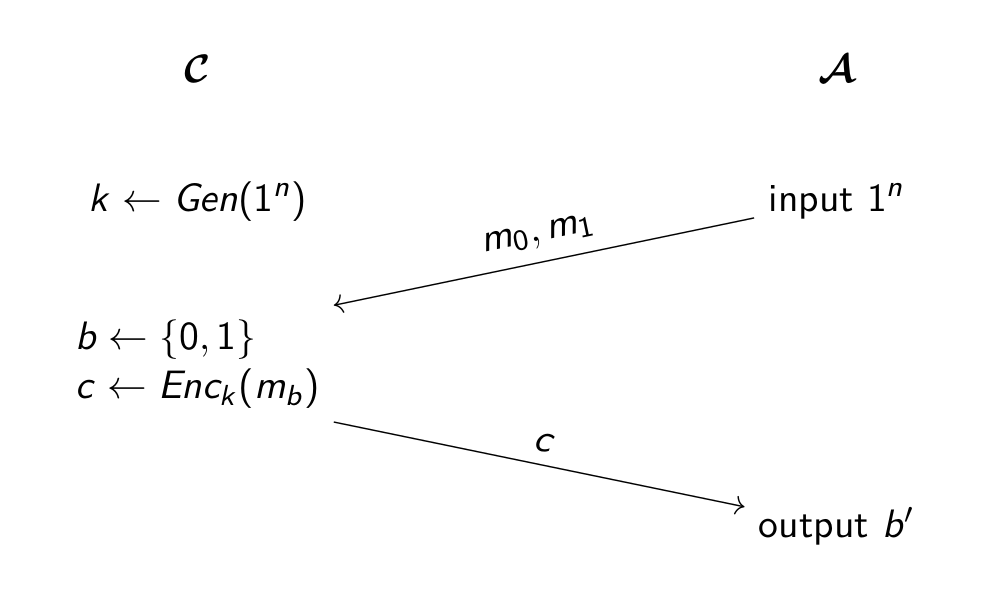
\includegraphics[width=.7\textwidth]{figures/eavesdropping_experiment.png}
\end{figure}
In the eavesdropping experiment, $\mathcal{C}$ first generates a random key $k$.
After that, $\mathcal{A}$ sends them two messages $m_0$ and $m_1$ for encryption with $|m_0| = |m_1|$.
$\mathcal{C}$ then chooses one of the two messages and encrypts it.
If $\mathcal{A}$ can tell which message $\mathcal{C}$ chose, the attack was successful.
If this happens with probability $0.5 + negligible$ the used cipher is secure.

\paragraph{Chosen-plaintext Attack}
\begin{figure}[H]
  \centering
  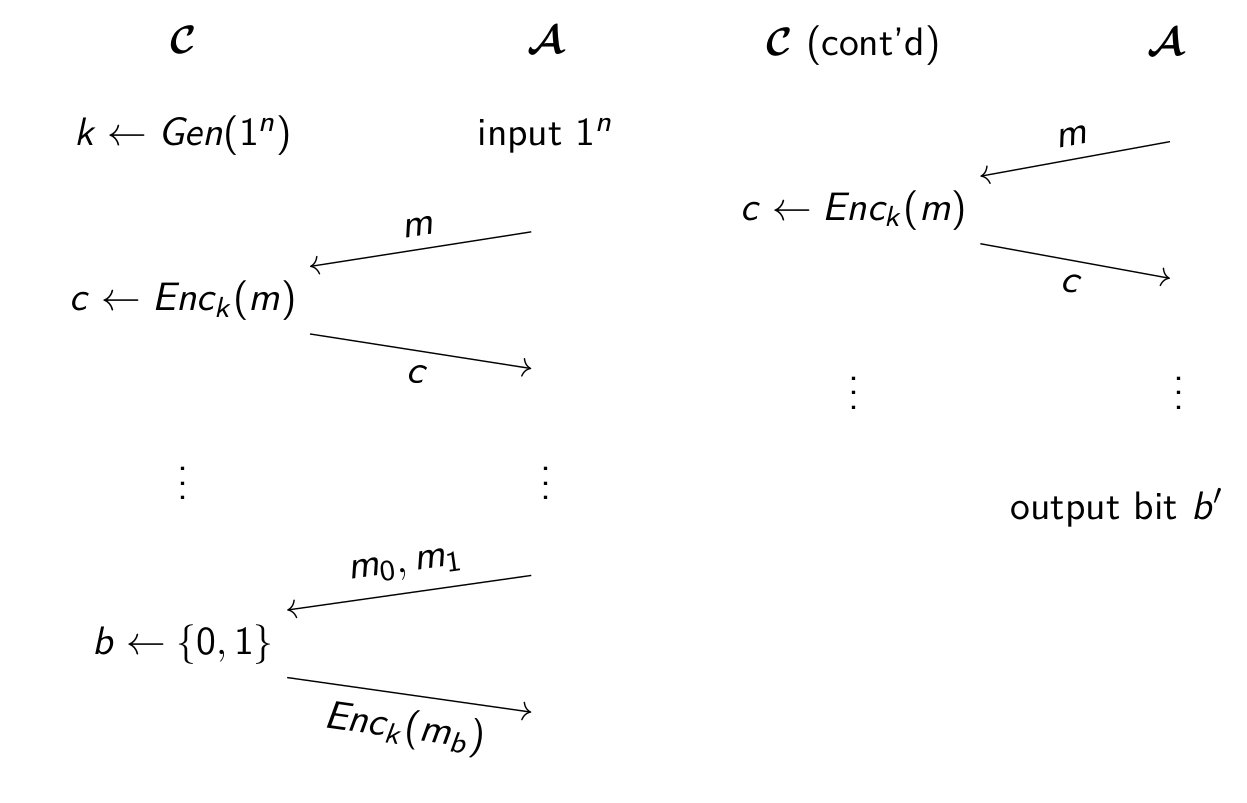
\includegraphics[width=.8\textwidth]{figures/cpa.png}
\end{figure}
In the chosen-plaintext attack the fist step again is that $\mathcal{C}$ generates a random key k.
$\mathcal{A}$ is then allowed to send an arbitrary amount of messages to $\mathcal{C}$ who will encrypt and send them back to $\mathcal{A}$ which means that $\mathcal{C}$ is an ``oracle'' for $\mathcal{A}$.
At some point, $\mathcal{A}$ will send two messages $m_0$ and $m_1$ of equal length of which $\mathcal{C}$ chooses one, encrypts it and sends the result back to $\mathcal{A}$.
$\mathcal{A}$ is then again allowed to use $\mathcal{C}$ as oracle for an arbitray amount of messages and if they are at some point able to tell which message ($m_0$ or $m_1$) $\mathcal{C}$ encrypted, the attack is successful.


\subsubsection{Block and Stream Ciphers}
A block cipher encrypts and decrypts inputs of length $n$ to outputs of length $n$ ($\Rightarrow$ block length $n$).
A steam cipher on the other hand generates a random bitstream with arbitrary length, called keystream, that is xored to the plain text to encrypt and decrypt.\\
The most advisable cipher to use is probably the AES block cipher.
It is well tested and proven to be (mostly) secure and hardware supported what makes it quite fast ($>2GB/s$ with HW support, $200Mbit/s$ without).

\subsubsection{Modes of Encryption}
Modes of encryption are necessary to handle messages of variable length with block ciphers.
The plaintext therefore is split into parts of length equal to the cipher block length.
If the last block is shorter than the block length, we add padding.

\paragraph{Electronic Code Book Mode (ECB)}
\begin{figure}[H]
  \centering
  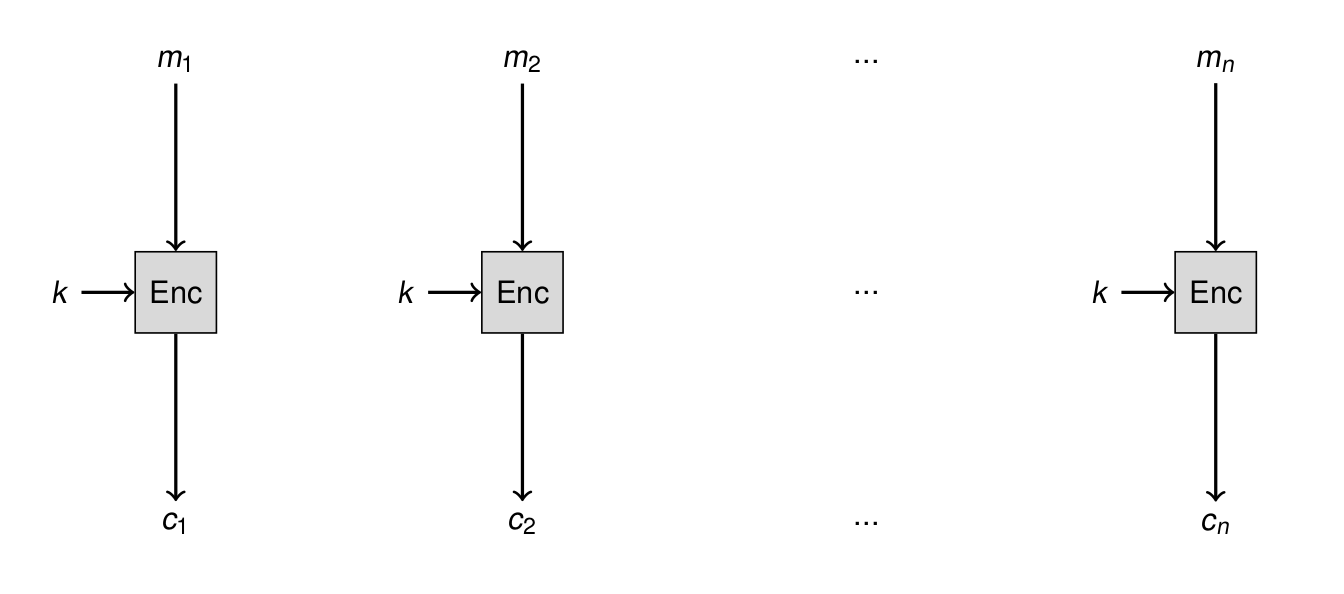
\includegraphics[width=.8\textwidth]{figures/ecb.png}
\end{figure}
In ECB, every plaintext block is encrypted with the unmodified key as input.
The problem thereby is that identical plaintext blocks result in the same ciphertext blocks.
\begin{figure}[H]
  \centering
  
\includegraphics[width=.8\textwidth]{figures/ecb_problem.png}
\end{figure}

\paragraph{Cipher Block Chaining Mode (CBC)}
\begin{figure}[H]
  \centering
  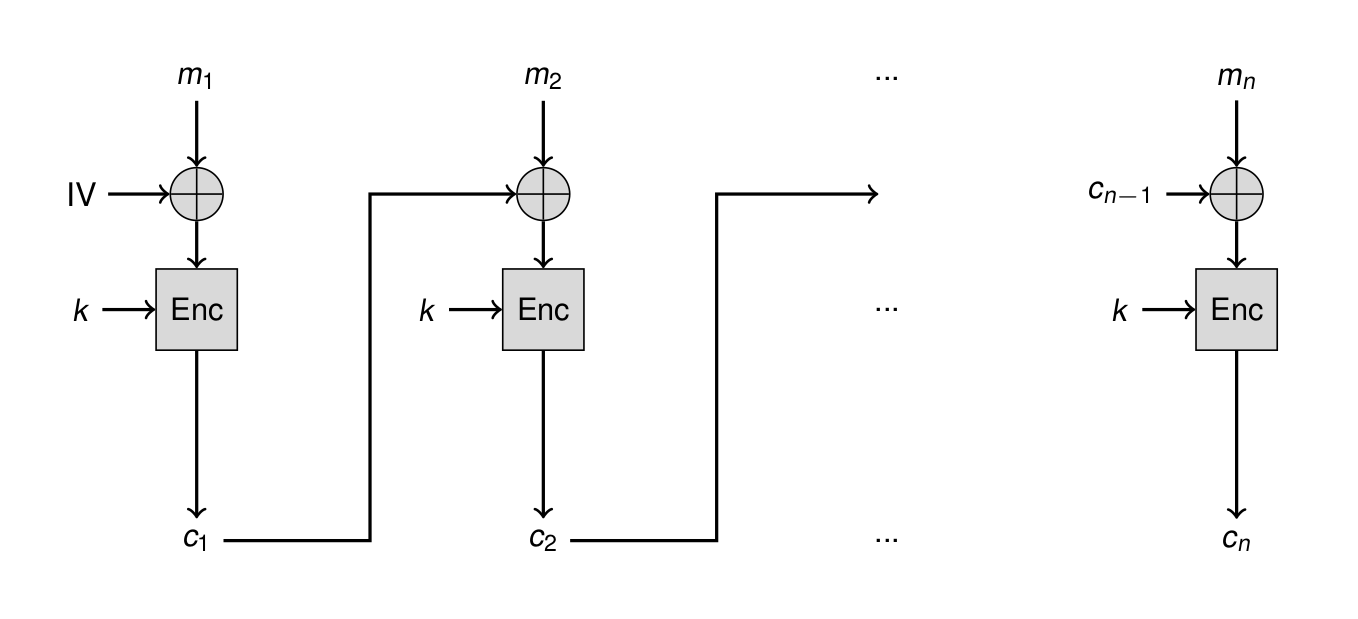
\includegraphics[width=.8\textwidth]{figures/cbc_encrypt.png}
  \caption{CBC Encrypt}\label{fig:cbc_encrypt}
\end{figure}
CBC uses the ciphertext from the previous block xored with the current message block and the unmodified key k as inputs of the encryption function $c_i = Enc_k(c_{i-1} \oplus m_i)$.
For the first message, where no previous cipher block is available, an initialization vector (IV) is used which may be sent in plaintext and is fresh for every massage (or packet if the message is split across multiple packets).\\
Compared to ECB, the advantage is that equal plaintext blocks/messages are not encrypted to the same ciphertext blocks/messages.
\begin{figure}[H]
  \centering
  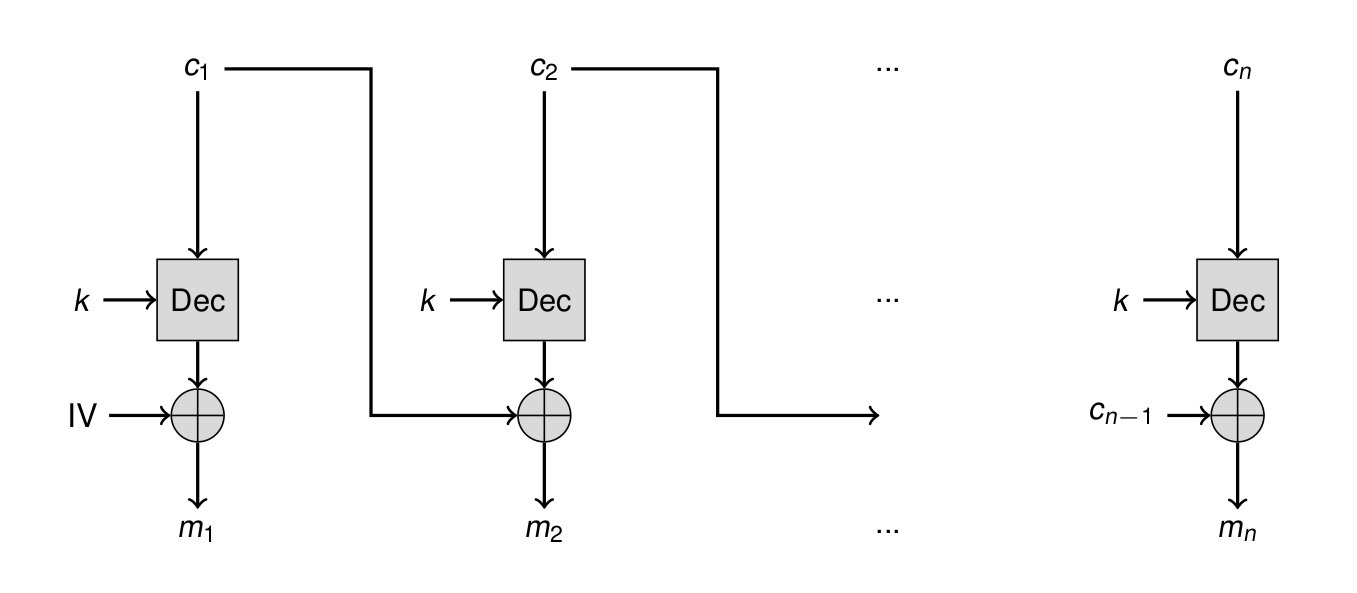
\includegraphics[width=.8\textwidth]{figures/cbc_decrypt.png}
  \caption{CBC Decrypt}
\end{figure}
Decryption is defined by $m_i = c_{i-1} \oplus Dec_k(c_i)$.

\paragraph{Output Feedback Mode (OFB)}
\begin{figure}[H]
  \centering
  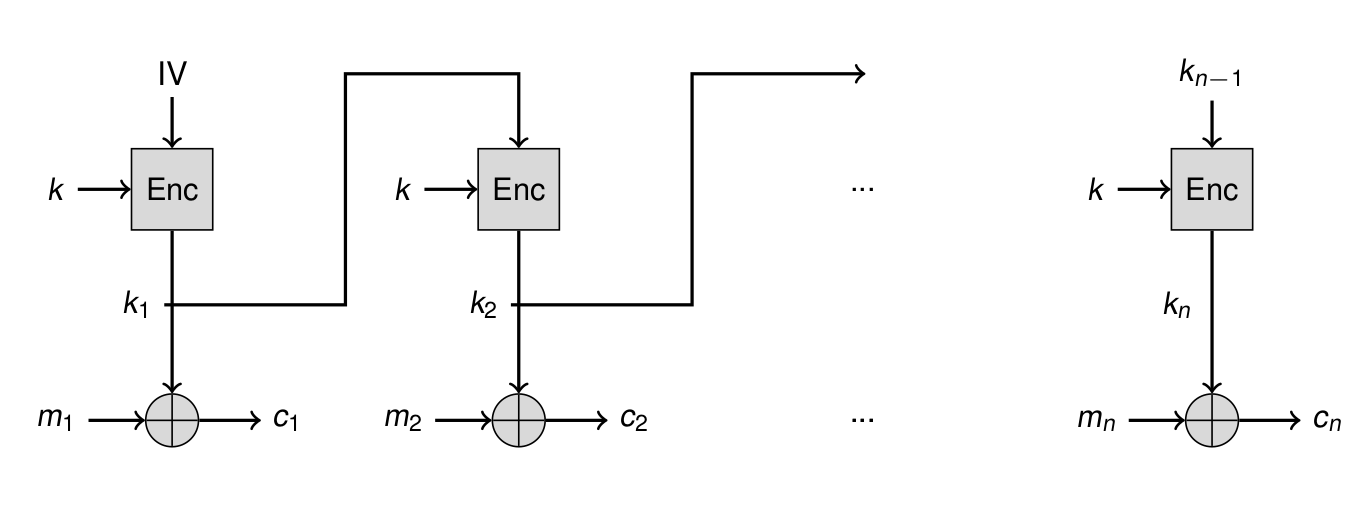
\includegraphics[width=.8\textwidth]{figures/ofb_encrypt.png}
  \caption{OFB Encrypt}
\end{figure}
OFB transforms a block cipher into a stream cipher.
In step $i$, it takes cipher key $k_{i-1}$ form the previous step and encrypts it with the key k.
This cipher key $k_i$ is then xored with the corresponding plaintext block $m_i$ to calculate the ciphertext $c_i$.
In the first step an IV is used as $k_{i-1}$.

\begin{figure}[H]
  \centering
  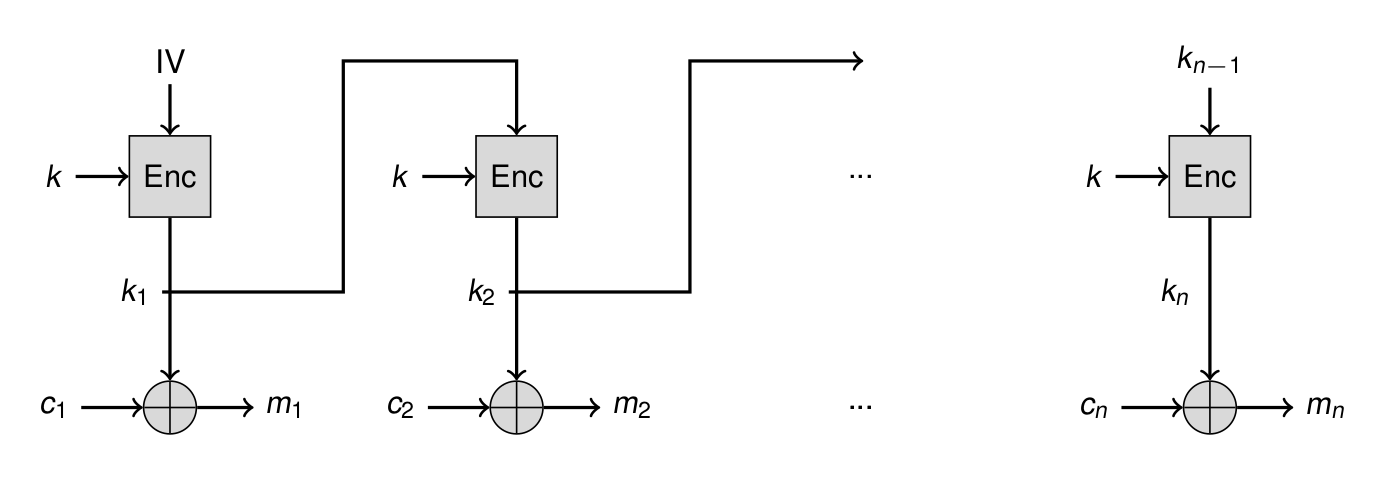
\includegraphics[width=.8\textwidth]{figures/ofb_decrypt}
  \caption{OFB Decrypt}
\end{figure}
Decryption is the same procedure except that the key stream is xored with the cipher text blocks.

\paragraph{Counter Mode (CTR)}
\begin{figure}[H]
  \centering
  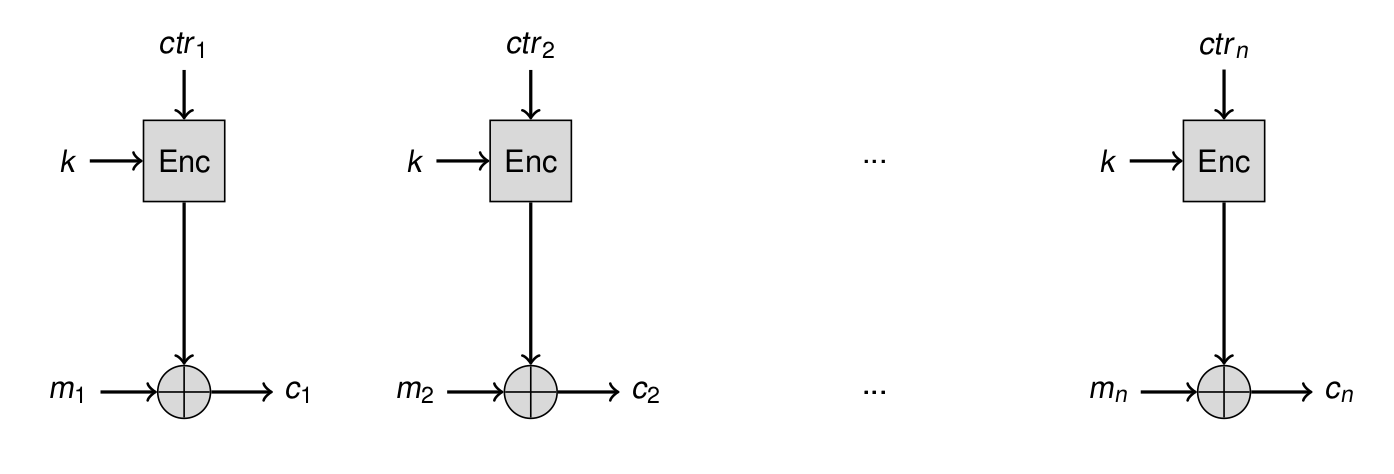
\includegraphics[width=.8\textwidth]{figures/ctr_encrypt}
  \caption{CTR Encrypt}
\end{figure}
In step $i$, CTR encrypts a counter $ctr_i = IV || i$ with key k and xors the result with the plaintext block $m_i$.
Like OFB, CTR also transforms block ciphers into stream ciphers.

\begin{figure}[H]
  \centering
  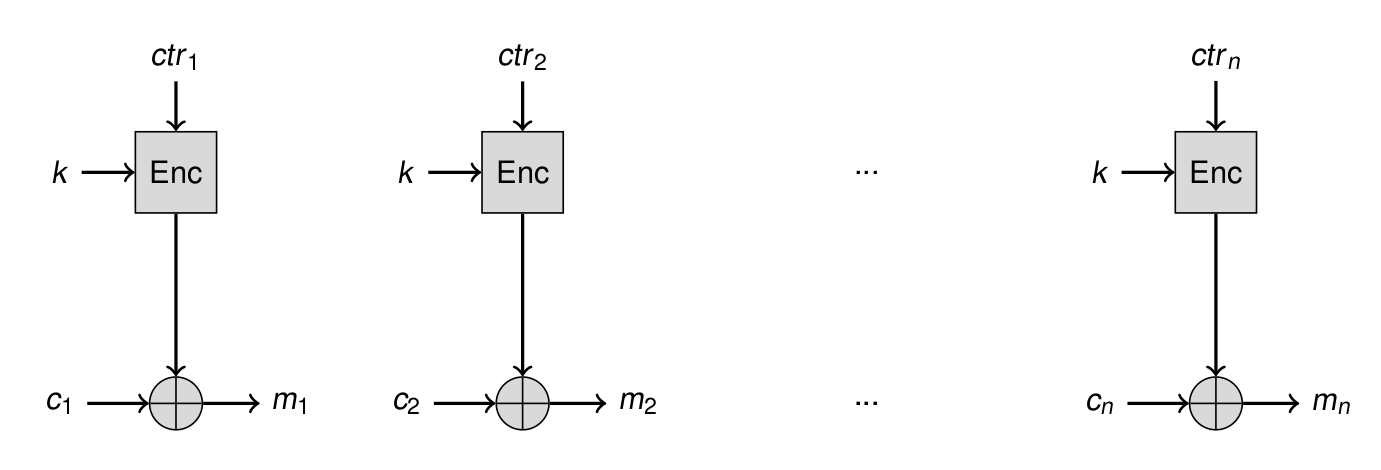
\includegraphics[width=.8\textwidth]{figures/ctr_decrypt.png}
  \caption{CTR Decrypt}
\end{figure}
Decryption is done by $m_i = Enc_k(ctr_i) \oplus c_i$.

\subsubsection{Message Authentication Code (MAC)}
MACs are used in symmetric cryptography to ensure message authenticity but do not provide replay protection.
They are transmitted with the message $\langle m,t \rangle$.
In practice, MACs are either based on hash functions (HMAC), CBC or included in the encryption (authenticated encryption modes).

We define the following terminology:
\begin{itemize}[noitemsep,topsep=0pt]
  \item Key $k \leftarrow Gen(1^n)$
  \item Tag $t \leftarrow Mac_k(m)$
  \item Verification $b := Vrfy_k(m,t)$ where $b=1$ means valid and $b=0$ invalid
\end{itemize}

We define a MAC as secure, if it withstands the adaptive chosen-message attack.

\paragraph{Adaptive Chosen-message Attack}
\begin{figure}[H]
  \centering
  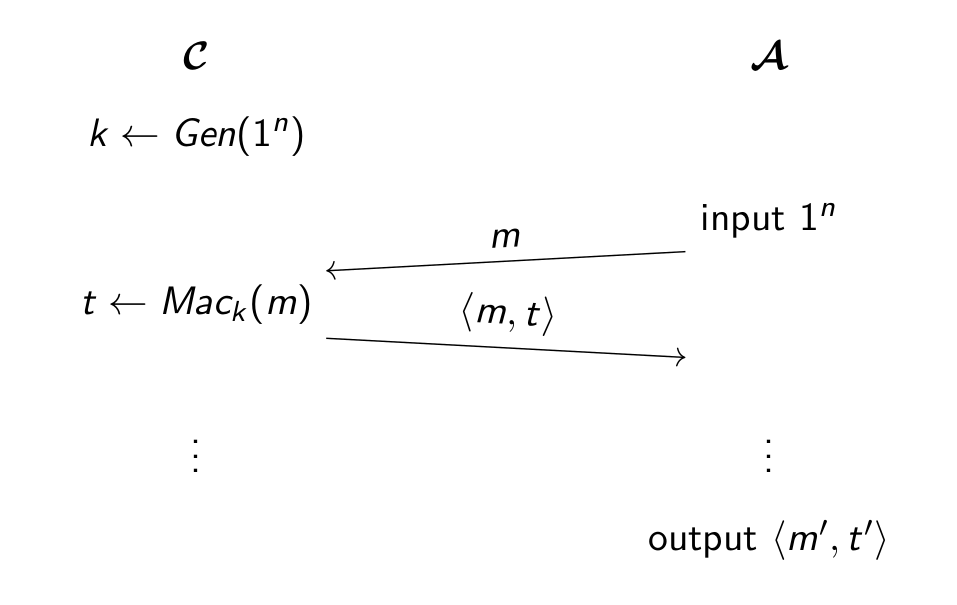
\includegraphics[width=.7\textwidth]{figures/adaptive_chosen-message_attack.png}
\end{figure}
In the adaptive chosen-message attack $\mathcal{C}$ first generates a random key $k$.
$\mathcal{A}$ then sends an arbitrary amount of messages to $\mathcal{C}$ for which they answer with a message consisting of the original message and a tag $t$.
At some point, $\mathcal{A}$ will generate a message-tag pair $\langle m',t' \rangle$ where $m$ was not previously sent to $\mathcal{C}$
The attack is successful, iff $Vrfy_k(m',t') = 1$, so if $\mathcal{A}$ was able to generate a valid MAC tag for a new message.

\paragraph{Hash MAC (HMAC)}
HMAC uses cryptographic hash functions to calculate the MAC\@.
It is calculated with
\begin{equation*}
  t = H(K \oplus opad~|~H(K \oplus ipad | m))
\end{equation*}
To note here is that $K$ is first extended to the block length required for the input of the hash function by appending zeros.
$opad$ and $ipad$ are arbitrary values with the restriction that they have a large Hemming distance to each other.\\
Another note: $H(K~|~m)$, $H(m~|~K)$ or $H(K~|~p~|~m~|~K)$ are not secure.

\paragraph{CBC-MAC}
CBC-MAC encrypts the message to authenticate with another key than used for encryption and uses the last ciphertext block as MAC\@.
CBC is shown in Figure~\ref{fig:cbc_encrypt}.
If the length of a message is not known or no other protection exists, CBC-MAC can be prone to length extension attacks.
CMAC resolves this.

\paragraph{CMAC}
CMAC is an improved version of CBC-MAC which has to keys, calculated from the shared key, where one is used for xoring with complete bocks before encryption and the other one for incomplete blocks.
XCBC-MAC is another improvement of this where the two keys are input to the algorithm and not derived from k.

\subsubsection{Combining Confidentiality and Authentication}
Generally the best approach to combine confidentiality and authentication is to first encrypt and then authenticate, i.e.\ $c \leftarrow Enc_{k_1}(m)$, $t \leftarrow Mac_{k_2}(c)$ and transmit $\langle c,t \rangle$.

\subsection{Asymmetric Cryptography}
In asymmetric cryptography, the two communication partners no longer have one shared key, but each participant has a key pair.
A private/secure key (sk) that is only known to one person and is used for decryption and message signing and a public key (pk) that can be published and is used for encryption and message verification.
Asymmetric cryptography is based on mathematical problems which are believed to be hard (e.g.\ integer factorization).
It only needs an authenticated channel to exchange keys of which less amounts are required than in the symmetric setting.
It is orders of magnitudes slower though.

\subsubsection{Public-key Encryption Scheme}
\begin{enumerate}
  \item $(pk,sk) \leftarrow Gen(1^n)$
  \item Encryption with public key: $c \leftarrow Enc_{pk}(m)$
  \item Decryption with private key: $m := Dec_{sk}(c)$
\end{enumerate}

\paragraph{RSA}
Key generation in RSA is done with the following procedure:
\begin{enumerate}
  \item $(N,p,q) \leftarrow GenModulus(1^n)$
  \item $\phi(N) := (p-1)(q-1)$
  \item find $e$: $\gcd(e,\phi(N)) = 1$
  \item $d := [e^{-1} \mod \phi(N)]$
  \item $pk = \langle N,e \rangle$
  \item $sk = \langle N,d \rangle$
\end{enumerate}

Encryption then is defined as $RSA_{pk}(y) := [y^e \mod N]$ and decryption as $RSA_{sk}(y) = [z^d \mod N]$.

\paragraph{Chosen-ciphertext Attack (CCA)}
An asymmetric encryption scheme is considered secure if it withstands CCA\@.
\begin{figure}[H]
  \centering
  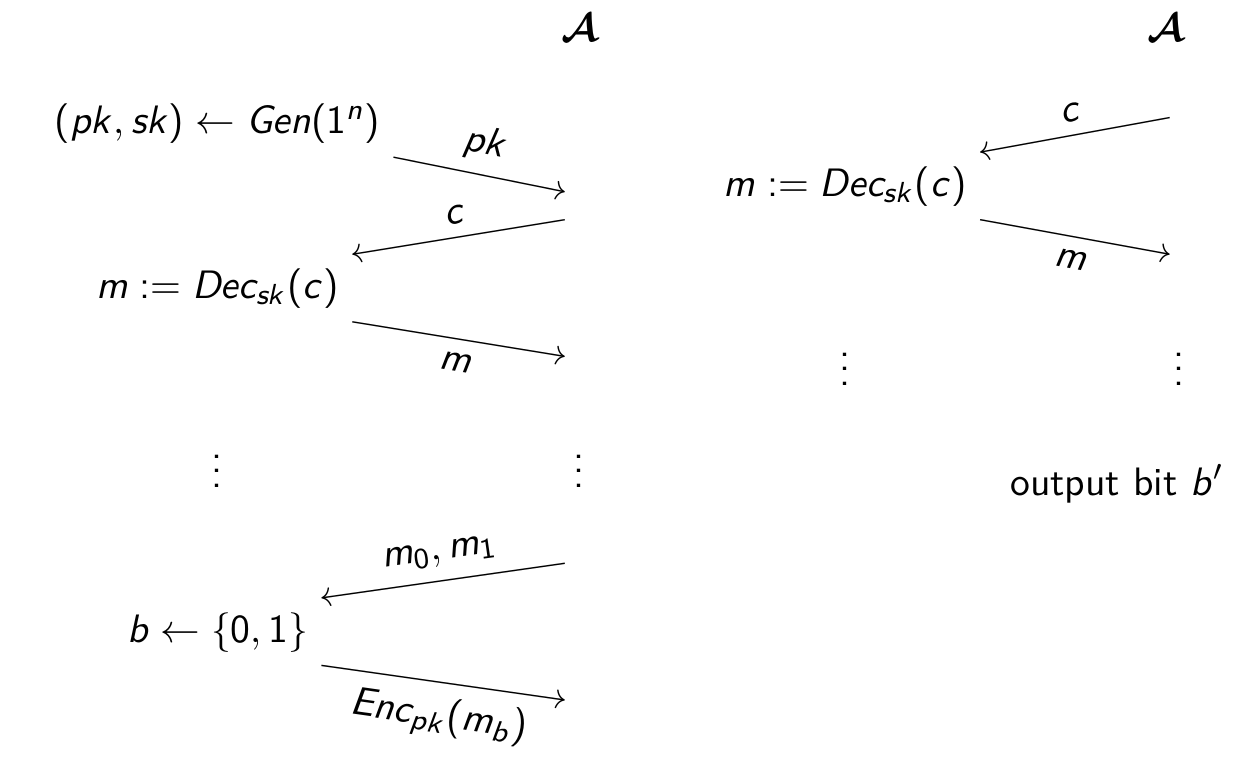
\includegraphics[width=.8\textwidth]{figures/cca.png}
\end{figure}
CCA is quite similar to CPA except $\mathcal{A}$ sends ciphertext messages to $\mathcal{C}$ for probing instead of plaintext ones.
A restriction not depicted in the illustration above is that $\mathcal{A}$ may not request a decryption for $Enc_{pk}(m_b)$ itself.
\newpage

\paragraph{Optimal Asymmetric Encryption Padding (OAEP)}
OAEP is a padding scheme for asymmetric encryption depicted below.
\begin{figure}[H]
  \centering
  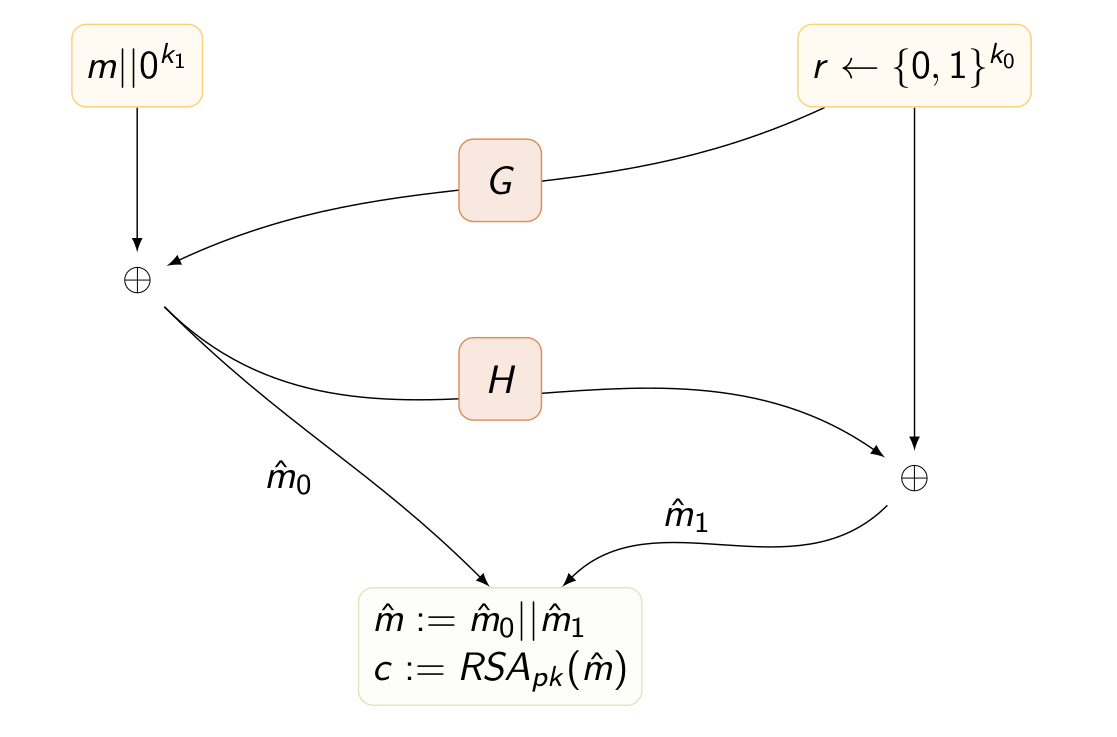
\includegraphics[width=.7\textwidth]{figures/oaep.png}
\end{figure}

RSA used in conjunction with OAEP is secure under CCA\@.

\subsubsection{Signature Scheme}
\begin{enumerate}
  \item $(pk,sk) \leftarrow Gen(1^n)$
  \item Signature generation with private key: $\sigma \leftarrow Sign_{sk}(m)$
  \item Signature verification with public key: $b := Vrfy_{pk}(m,\sigma)$ where $b = 1$ means valid and $b = 0$ invalid
\end{enumerate}
Signatures are often slower than their MAC relatives and provide non-repudiation.
A signature scheme is considered secure if it withstands the adaptive chosen-message attack.
\newpage

\paragraph{RSASSA-PSS}
RSASSA-PSS is a signature scheme that uses RSA\@.
\begin{figure}[H]
  \centering
  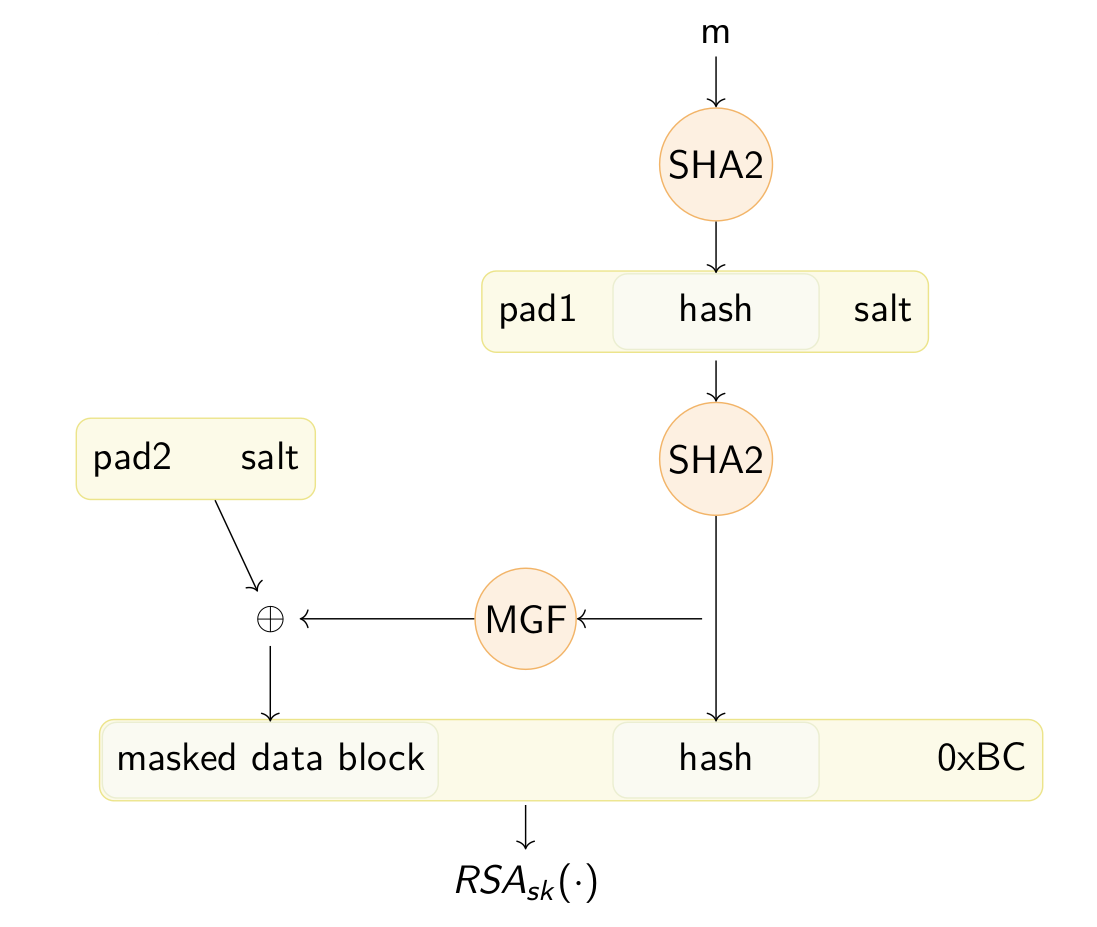
\includegraphics[width=.8\textwidth]{figures/rsassa-pss.png}
\end{figure}
RSASSA-PSS is secure under adaptive chosen-message attack and breaking it would mean that RSA is broken.

\subsection{Hybrid Approach}
Since public key cryptography is slower than secret key cryptography, a hybrid approach is often advisable.
Public-key cryptography is used to protect a shared key (session key) that is used for any further communication via secret-key cryptography.
They private key for the key exchange is called long-term key.\\

\textbf{Perfect forward secrecy} is often an important property of this approach.
It states that if an attacker gains access to the long-term key or the session key, they should not be able to decrypt messages of past sessions.\\

A common strategy is to use a signed Diffie-Hellman key exchange and a secret-key authenticated encryption scheme for communication.
To guarantee perfect forward secrecy, DH keys have to be calculated for every connection and old keys have to be wiped.
\newpage

\subsubsection{Diffie-Hellman Key Exchange (DH)}
\begin{figure}[H]
  \centering
  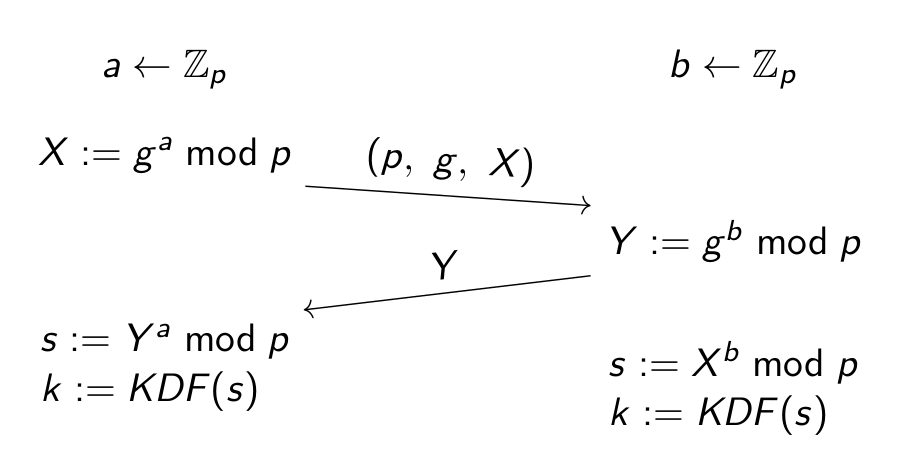
\includegraphics[width=.7\textwidth]{figures/diffie-hellmann.png}
\end{figure}
In the first step of the DH key exchange, communication partner A selects a prime $p$, a generator $g$ which is a primitive root for the cyclic group of $\mathds{Z}_p$ and a random number $a \in \mathds{Z}_p$.
A then calculates $X = g^a \mod p$ and sends it with $p$ and $g$ to B.
B also chooses a random number $b \in \mathds{Z}_p$ and calculates $Y = g^b \mod p$ which they send back to A.
Both can then calculate the key $k$ by $k = Y^a = g^{ba} = g^{ab} = X^b~\mod p$.

\newpage

% Needs to be enabled when there are any references.
% \clearpage
% \addcontentsline{toc}{section}{\refname}
% \printbibliography

\end{document}
